\documentclass[
11pt, % The default document font size, options: 10pt, 11pt, 12pt
%codirector, % Uncomment to add a codirector to the title page
]{charter} 


% El títulos de la memoria, se usa en la caratula y se puede usar el cualquier lugar del documento con el comando \ttitle
\titulo{Sistema de monitoreo de \textit{Rhynchophorus ferrugineus} en palmeras de Montevideo} 


% Nombre del posgrado, se usa en la caratula y se puede usar el cualquier lugar del documento con el comando \degreename
% \posgrado{Carrera de Especialización en Sistemas Embebidos} 
%\posgrado{Carrera de Especialización en Internet de las Cosas} 
\posgrado{Carrera de Especialización en Inteligencia Artificial}
%\posgrado{Maestría en Sistemas Embebidos} 
%\posgrado{Maestría en Internet de las cosas}

% Tu nombre, se puede usar el cualquier lugar del documento con el comando \authorname
% IMPORTANTE: no omitir titulaciones ni tildación en los nombres, también se recomienda escribir los nombres completos (tal cual los tienen en su documento)
\autor{Ing. Bruno Masoller}

% El nombre del director y co-director, se puede usar el cualquier lugar del documento con el comando \supname y \cosupname y \pertesupname y \pertecosupname
\director{Ing. Juan Ignacio Cavalieri}
\pertenenciaDirector{FIUBA} 
\codirector{} % para que aparezca en la portada se debe descomentar la opción codirector en los parámetros de documentclass
\pertenenciaCoDirector{FIUBA}

% Nombre del cliente, quien va a aprobar los resultados del proyecto, se puede usar con el comando \clientename y \empclientename
\cliente{Ing. Agr. Alfonso Arcos}
\empresaCliente{Intendencia de Montevideo}
 
\fechaINICIO{15 de octubre de 2024}		%Fecha de inicio de la cursada de GdP \fechaInicioName
\fechaFINALPlan{03 de diciembre de 2024} 	%Fecha de final de cursada de GdP
\fechaFINALTrabajo{junio de 2025}	%Fecha de defensa pública del trabajo final


\begin{document}

\maketitle
\thispagestyle{empty}
\pagebreak


\thispagestyle{empty}
{\setlength{\parskip}{0pt}
  \tableofcontents{}
}
\pagebreak

\section*{Registros de cambios}
\label{sec:registro}


\begin{table}[ht]
  \label{tab:registro}
  \centering
  \begin{tabularx}{\linewidth}{@{}|c|X|c|@{}}
    \hline
    \rowcolor[HTML]{C0C0C0}
    Revisión & \multicolumn{1}{c|}{\cellcolor[HTML]{C0C0C0}Detalles de los cambios realizados}       & Fecha                       \\ \hline
    0        & Creación del documento                                                                & \fechaInicioName            \\ \hline
    1        & Se completa hasta el punto 5 inclusive                                                & {29} de {octubre} de 2024   \\ \hline
    2        & Se corrige secciones 1, 2, 3, 4 y 5. \newline Se completa hasta el punto 9 inclusive. & {05} de {noviembre} de 2024 \\ \hline
    3        & Se corrige secciones 1, 2, 6 y 9. \newline Se completa hasta el punto 12 inclusive.   & {12} de {noviembre} de 2024 \\ \hline
    %4      & Se completa el plan	                                 & {día} de {mes} de 202X \\ \hline

    % Si hay más correcciones pasada la versión 4 también se deben especificar acá
  \end{tabularx}
\end{table}

\pagebreak

\section*{Acta de constitución del proyecto}
\label{sec:acta}

\begin{flushright}
  Buenos Aires, \fechaInicioName
\end{flushright}

\vspace{2cm}

Por medio de la presente se acuerda con el \authorname\hspace{1px} que su Trabajo Final de la \degreename\hspace{1px} se titulará ``\ttitle'' y consistirá en la presentación de una prueba de concepto de un sistema de monitoreo de la plaga \textit{Rhynchophorus ferrugineus} en palmeras de Montevideo. El trabajo tendrá un presupuesto preliminar estimado de 600 horas y un costo estimado de USD 28756, con fecha de inicio el \fechaInicioName\hspace{1px} y fecha de presentación pública en \fechaFinalName.

Se adjunta a esta acta la planificación inicial.

\vfill

% Esta parte se construye sola con la información que hayan cargado en el preámbulo del documento y no debe modificarla
\begin{table}[ht]
  \centering
  \begin{tabular}{ccc}
    \begin{tabular}[c]{@{}c@{}}Dr. Ing. Ariel Lutenberg \\ Director posgrado FIUBA\end{tabular} & \hspace{2cm} & \begin{tabular}[c]{@{}c@{}}\clientename \\ \empclientename \end{tabular} \vspace{2.5cm} \\
    \multicolumn{3}{c}{\begin{tabular}[c]{@{}c@{}} \supname \\ Director del Trabajo Final\end{tabular}} \vspace{2.5cm}                                                                                   \\
  \end{tabular}
\end{table}

\section{1. Descripción técnica-conceptual del proyecto a realizar}
\label{sec:descripcion}

En Montevideo, hay alrededor de 25.000 palmeras, que forman una parte esencial del paisaje urbano y contribuyen al equilibrio del ecosistema local. Desde 2010, la plaga del \textit{Rhynchophorus ferrugineus}, conocido comúnmente como “picudo rojo” (ver figura \ref{fig:picudo-rojo}), ha estado propagándose por América, llegando a Uruguay en 2022. Esta plaga supone una amenaza grave para las palmeras, ya que las larvas de este escarabajo se alimentan de su tejido interno, causando el colapso estructural de los árboles en un período de entre 8 y 10 meses.

La infestación del picudo rojo no solo tiene consecuencias ecológicas, sino también económicas. La caída de palmeras infectadas puede provocar daños a personas y propiedades, especialmente durante los fuertes vientos que afectan a Montevideo. Además, la eliminación de estos árboles infestados implica un costo aproximado de 1.000 dólares estadounidenses por unidad.

\begin{figure}[H]
  \centering
  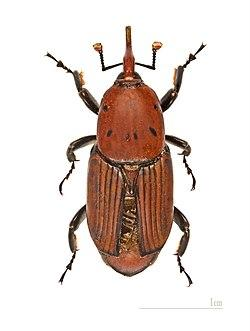
\includegraphics[width=.30\textwidth]{./Figuras/picudo-rojo.png}
  \caption{Rhynchophorus ferrugineus.}
  \label{fig:picudo-rojo}
\end{figure}

Actualmente, el método principal método de detección que utiliza la Intendencia de Montevideo (IM), consiste en la inspección visual presencial en lugares donde se sospecha la presencia de la plaga o se ha reportado por parte de particulares. La IM también tiene otros métodos de detección, como lo son trampas colocadas en puntos claves de la ciudad que permiten observar el desplazamiento de la plaga.

El servicio de Áreas Verdes es el principal encargado del tratamiento de la plaga del picudo rojo y gestiona sectores clave, como el de arbolado, que representa una de las primeras líneas de defensa. Este servicio proporciona diversos datos y colabora estrechamente con otras áreas importantes para la gestión de la plaga, como los servicios de Geomática e Informática. Entre los datos disponibles, se incluye la ubicación de todas las palmeras en el sistema de información geográfica de la IM. Además, el servicio de Geomática cuenta con drones que permiten obtener imágenes de ortomosaicos bajo demanda (ver figura \ref{fig:imagen-dron-y-avion}), las cuales pueden ser solicitadas por el servicio de Áreas Verdes. Estos ortomosaicos alcanzan una resolución espacial de 3 cm por píxel en el rango espectral RGB. Adicionalmente, se realizan vuelos que cubren toda la ciudad de Montevideo, lo cual permite la generación de ortomosaicos de alta resolución en dicho rango espectral.

\begin{figure}[H]
  \centering
  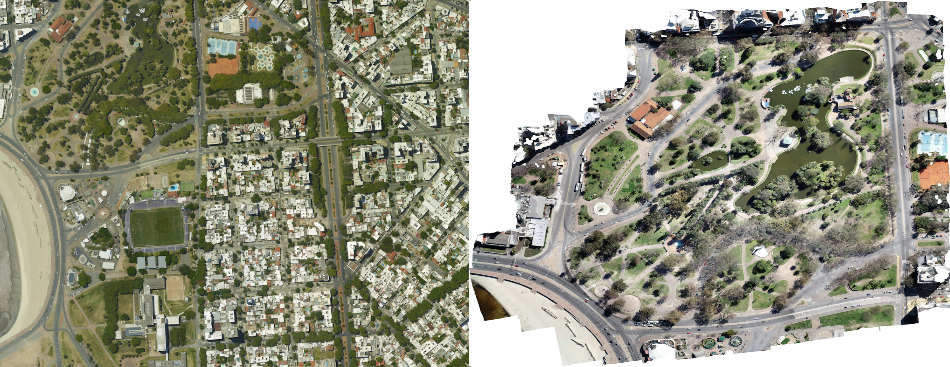
\includegraphics[width=.95\textwidth]{./Figuras/imagen-dron-y-avion.png}
  \caption{Fotografías ortorectificadas de un vuelo de avión y dron, respectivamente.}
  \label{fig:imagen-dron-y-avion}
\end{figure}

Se ha demostrado la viabilidad de detectar la plaga utilizando imágenes capturadas con Google Street View (a nivel de suelo)\cite{kagan2024}. Además, existen datos que avalan la identificación de palmeras en imágenes obtenidas mediante drones, con resoluciones similares a las del servicio de Geomática de la IM. Sin embargo, la detección directa de la plaga en imágenes aéreas en el rango visible sigue siendo un desafío, aunque algunos estudios han explorado el uso del índice de vegetación e imágenes en la banda infrarroja para este fin\cite{delalieux2023}.

Este proyecto propone un enfoque integral que conecta la información geoespacial gestionada por el servicio de Informática con los recursos de imágenes aéreas del servicio de Geomática. El objetivo es desarrollar una plataforma informática que mejore la eficiencia en el tratamiento de la plaga, especialmente en el proceso de inspección manual, mediante el uso de modelos de vanguardia en visión por computadora y aprendizaje profundo.

Como proyecto en general, se propone una plataforma como el de la siguiente figura \ref{fig:diagrama-inicial-solucion}.

\begin{figure}[H]
  \centering
  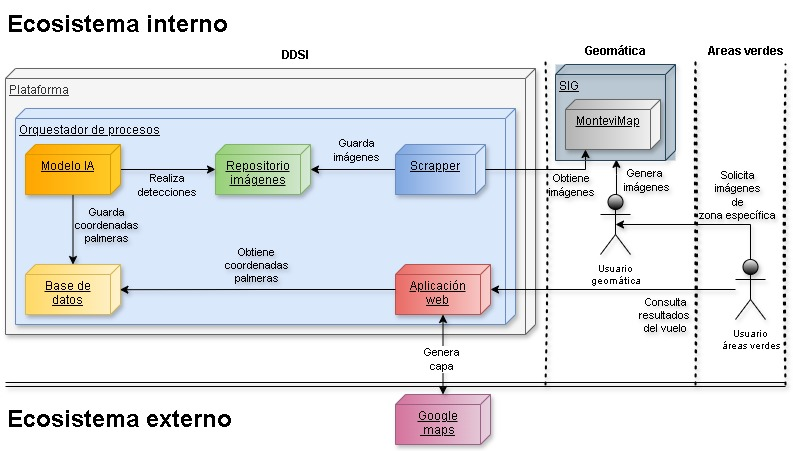
\includegraphics[width=.95\textwidth]{./Figuras/diagrama-inicial-solucion.jpg}
  \caption{Diagrama de la solución.}
  \label{fig:diagrama-inicial-solucion}
\end{figure}

La implementación de esta plataforma ofrece beneficios tanto económicos como ambientales para la IM. La detección temprana y tardía de la plaga puede reducir los costos de inspección presencial y optimizar el uso de drones, aprovechando su capacidad para cubrir grandes áreas. En particular, esta plataforma permitirá a la IM optimizar sus recursos en el manejo del picudo rojo, lo que reducirá los costos asociados a la remoción de palmeras, enfocará las inspecciones presenciales solo en casos excepcionales y permitirá la realización de vuelos programados de drones para maximizar su autonomía. Asimismo, validará un prototipo que puede extenderse a otros proyectos, que pueden contribuir a la preservación del entorno ecológico de la ciudad y a la seguridad de sus habitantes. Finalmente, se brinda la posibilidad de incorporar un módulo para la detección automática de palmeras en los vuelos aéreos.

\section{2. Identificación y análisis de los interesados}
\label{sec:interesados}

\begin{table}[ht]
  %\caption{Identificación de los interesados}
  %\label{tab:interesados}
  \begin{tabularx}{\linewidth}{@{}|l|X|X|l|@{}}
    \hline
    \rowcolor[HTML]{C0C0C0}
    Rol           & Nombre y Apellido        & Organización    & Puesto                        \\ \hline
    Cliente       & \clientename             & \empclientename & Director sector arbolado      \\ \hline
    Impulsor      & Msc. Ing. Juan Prada     & \empclientename & Gerente ciudades inteligentes \\ \hline
    Responsable   & \authorname              & \empclientename & Alumno                        \\ \hline
    Orientador    & \supname                 & \pertesupname   & Director del trabajo final    \\ \hline
    Usuario final & Usuarios de áreas verdes & \empclientename & Administrativo                \\ \hline
  \end{tabularx}
\end{table}

Descripción de los interesados:
\begin{itemize}
  \item Cliente: aunque no cuenta con conocimientos técnicos avanzados en visión por computadora, el cliente es experto en la problemática del picudo rojo y posee habilidades en gestión e implementación de soluciones diversas. Es uno de los principales promotores del proyecto y tiene un alto interés en su éxito.

  \item Impulsor: el Gerente de Ciudades Inteligentes cuenta con conocimientos sólidos tanto en inteligencia artificial como en gestión de proyectos. Es un impulsor clave de estas iniciativas, que se alinean con la visión estratégica de la organización.

  \item Orientador: el \supname tiene un conocimiento profundo en visión por computadora, particularmente en el contexto de esta problemática. Además, es profesor de \pertesupname en la asignatura de Visión por Computadora II, brindando apoyo técnico y conceptual al proyecto.

  \item Usuario final: los usuarios finales son técnicos de áreas verdes capacitados para identificar visualmente la plaga en las palmeras. Realizan el análisis de datos, gestionan la georreferenciación de las palmeras y, cuando es necesario, llevan a cabo inspecciones de campo.
\end{itemize}

\section{3. Propósito del proyecto}
\label{sec:proposito}

Proveer una prueba de concepto (POC) del componente de inteligencia artificial de una plataforma informática, alineada con la visión de la IM (\textit{Montevideo más verde}), que permita mejorar la eficiencia en la detección del \textit{Rhynchophorus ferrugineus}, utilizando técnicas avanzadas de visión por computadora y aprendizaje profundo.

\section{4. Alcance del proyecto}
\label{sec:alcance}

El alcance de la etapa inicial del proyecto incluye:
\begin{itemize}
  \item Investigar la viabilidad de la detección del \textit{Rhynchophorus ferrugineus} mediante técnicas de visión por computadora en dominios multiespectrales.
  \item Desarrollar un modelo de visión por computadora que permita detectar el \textit{Rhynchophorus ferrugineus} en palmeras de Montevideo.
  \item Gestionar el proceso de etiquetado de datos.
  \item Escribir una memoria con los resultados del proyecto.
\end{itemize}

En esta etapa, el proyecto no incluye:
\begin{itemize}
  \item La detección de la plaga y palmeras mediante imágenes de vuelos por aviones.
  \item Identificación del grado de infección de las palmeras, sino su clasificación binaria en infectadas y no infectadas.
  \item Otros componentes de la arquitectura presentada que no sea el modelo de visión por computadora.
  \item Las posibles extensiones de la plataforma.
  \item La gestión del ciclo de vida del modelo de detección.
  \item La evolución del sistema.
\end{itemize}

\section{5. Supuestos del proyecto}
\label{sec:supuestos}


Para el desarrollo del presente proyecto se supone que:

\begin{itemize}

  \item Se cuenta con disponibilidad horaria de al menos 20 horas semanales para realizar el proyecto.
  \item Se cuenta con imágenes de drones con resoluciones espaciales de al menos 3 cm/pixel.
  \item Se cuenta con voluntad del cliente para realizar el etiquetado de las imágenes.
  \item Se cuenta con la infraestructura necesaria para el despliegue de los componentes de software.
  \item Se cuenta con el apoyo de la IM para la ejecución del proyecto.
  \item Se cuenta con que se pueda detectar la plaga mediante imágenes RGB o infrarrojas (o combinación de ambas) obtenidas desde drones.
  \item Se cuenta con imágenes georeferenciadas.
  \item Se cuenta con mosaicos ortorectificados.

\end{itemize}

\section{6. Requerimientos}
\label{sec:requerimientos}

Para una mejor organización los requisitos se expresan utilizando una metodología de rotulado contextual, donde cada uno se identifica según su nivel de afinidad y jerárquico.

La notación se realiza en lenguaje natural, siguiendo un formato estandarizado, donde se especifica el actor y luego la funcionalidad.

La organización jerárquica se toma del template de referencia de especificación de requisitos de software de la IEEE\cite{SRSTemplateIEE}.

Finalmente, se priorizan utilizando el método \textit{MoSCoW}\cite{moscowMethod}.

\begin{enumerate}
  \item Requisitos de interfaces internas:
        \begin{enumerate}
          \item Modelo de visión por computadora
                \begin{enumerate}[label={[RII-ModeloVPC-\arabic*]}, leftmargin=*]
                  \item (S) El modelo de visión por computadora debe proporcionar un servicio web que reciba una imagen y devuelva una estructura de datos con las detecciones y sus coordenadas.
                \end{enumerate}
          \item Visualizador de detecciones
                \begin{enumerate}[label={[RII-VisDetecciones-\arabic*]}, leftmargin=*]
                  \item (S) El visualizador de detecciones debe aceptar una imagen y la estructura de datos de las detecciones, mostrando la imagen compuesta con las detecciones realizadas.
                \end{enumerate}
        \end{enumerate}

  \item Requisitos de interfaces externas:
        \begin{enumerate}
          \item Gestor de datos
                \begin{enumerate}[label={[RF-GestorDatos-\arabic*]}, leftmargin=*]
                  \item (S) El gestor de datos debe ser accesible desde internet por los usuarios de áreas verdes.
                \end{enumerate}
          \item Visualizador de detecciones
                \begin{enumerate}[label={[RII-VisDetecciones-\arabic*]}, leftmargin=*]
                  \item (S) El visualizador de detecciones debe ser accesible desde internet por los usuarios de áreas verdes.
                \end{enumerate}
        \end{enumerate}

  \item Requisitos funcionales:
        \begin{enumerate}
          \item Modelo de visión por computadora
                \begin{enumerate}[label={[RF-ModeloVPC-\arabic*]}, leftmargin=*]
                  \item (M) El modelo de visión debe ser capaz de generar predicciones a partir de una imagen proporcionada.
                  \item (M) El modelo de visión debe identificar palmeras en imágenes aéreas de forma precisa.
                  \item (M) El modelo de visión debe clasificar automáticamente las palmeras en dos categorías: infectadas y no infectadas.
                \end{enumerate}
          \item Visualizador de detecciones
                \begin{enumerate}[label={[RF-VisDetecciones-\arabic*]}, leftmargin=*]
                  \item (C) El visualizador de detecciones debe permitir la visualización de una imagen junto con sus detecciones.
                \end{enumerate}
          \item Gestor de datos
                \begin{enumerate}[label={[RF-GestorDatos-\arabic*]}, leftmargin=*]
                  \item (S) El gestor de datos debe incluir una herramienta para el etiquetado de datos que permita al cliente etiquetar imágenes de drones.
                  \item (C) El gestor de datos debe almacenar los datos etiquetados en el repositorio de la Intendencia Municipal (IMNube).
                \end{enumerate}
        \end{enumerate}

  \item Requisitos del proceso:
        \begin{enumerate}
          \item Modelo de visión por computadora
                \begin{enumerate}[label={[RP-ModeloVPC-\arabic*]}, leftmargin=*]
                  \item (S) Se debe investigar el estado del arte en modelos de visión por computadora para la detección de la plaga.
                  \item (C) Se debe realizar una investigación sobre enfoques de detección de plagas mediante imágenes multiespectrales.
                \end{enumerate}
          \item Gestor de datos
                \begin{enumerate}[label={[RP-GestorDatos-\arabic*]}, leftmargin=*]
                  \item (C) Se deben investigar herramientas adecuadas para el etiquetado de datos.
                \end{enumerate}
        \end{enumerate}

  \item Requisitos de datos:
        \begin{enumerate}
          \item Gestor de datos
                \begin{enumerate}[label={[RDATA-GestorDatos-\arabic*]}, leftmargin=*]
                  \item (C) El sistema debe permitir al cliente etiquetar al menos 100 imágenes, asegurando un equilibrio entre las clases de palmeras infectadas y no infectadas.
                \end{enumerate}
        \end{enumerate}

  \item Requisitos de documentación:
        \begin{enumerate}
          \item Informe final
                \begin{enumerate}[label={[RDOC-InformeFinal-\arabic*]}, leftmargin=*]
                  \item (M) Se debe elaborar un informe final que incluya una presentación completa del proyecto y sus resultados.
                  \item (C) Se debe elaborar un informe de avance a mitad del tiempo asignado para el proyecto, detallando los progresos realizados.
                \end{enumerate}
        \end{enumerate}

  \item Requisitos de rendimiento:
        \begin{enumerate}
          \item Modelo de visión por computadora
                \begin{enumerate}[label={[RR-ModeloVPC-\arabic*]}, leftmargin=*]
                  \item (C) El modelo de visión por computadora debe mantener una precisión mínima del 90\% en la identificación de palmeras y un 80\% en la clasificación de infestación.
                  \item (C) El modelo de visión por computadora debe ser capaz de procesar imágenes capturadas en condiciones de iluminación variables.
                \end{enumerate}
        \end{enumerate}

  \item Requisitos de interfaces gráficas:
        \begin{enumerate}
          \item Visualizador de detecciones
                \begin{enumerate}[label={[RII-VisDetecciones-\arabic*]}, leftmargin=*]
                  \item (C) El visualizador de detecciones debe brindar un criterio de satisfacción de usabilidad mayor al 80\% para los usuarios.
                \end{enumerate}
        \end{enumerate}

  \item Requisitos de seguridad (\textit{security}):
        \begin{enumerate}
          \item Gestor de datos
                \begin{enumerate}[label={[RF-GestorDatos-\arabic*]}, leftmargin=*]
                  \item (S) El gestor de datos debe estar bajo un mecanismo de autorización de usuarios.
                \end{enumerate}
          \item Visualizador de detecciones
                \begin{enumerate}[label={[RII-VisDetecciones-\arabic*]}, leftmargin=*]
                  \item (S) El visualizador de datos debe estar bajo un mecanismo de autorización de usuarios.
                \end{enumerate}
        \end{enumerate}

  \item Requisitos de diseño:
        \begin{enumerate}
          \item Lenguaje
                \begin{enumerate}[label={[RD-ModeloVPC-\arabic*]}, leftmargin=*]
                  \item (C) El sistema debe ser implementado utilizando \textit{Python 3} para el procesamiento backend.
                  \item (C) El sistema debe ser implementado utilizando \textit{Angular} para el procesamiento frontend.
                  \item (C) El protocolo de comunicación de los servicios debe ser \textit{REST}.
                \end{enumerate}
        \end{enumerate}
\end{enumerate}

\section{7. Historias de usuarios (\textit{Product backlog})}
\label{sec:backlog}

Las historias de usuario contienen sus criterios de aceptación, y se ponderan según la complejidad, dificultad e incertidumbre.
El resultado final de puntos de historia, es el número de \textit{Fibonacci} superior más cercano.

Los actores involucrados son:

\begin{table}[ht]
  \begin{tabularx}{\linewidth}{@{}|l|X|X|l|@{}}
    \hline
    \rowcolor[HTML]{C0C0C0}
    Actor                                & Descripción                                                                                                                                                             \\ \hline
    Usuario técnico de la IM             & El usuario técnico de la IM es el responsable de realizar la implementación técnica del proyecto, lo que incluye todo lo relacionado con el ciclo de vida del software. \\ \hline
    Usuario del servicio de áreas verdes & El usuario del servicio de áreas verdes es el encargado de interactuar con el software en modalidad de "usuario final".                                                 \\ \hline
    Usuario responsable del proyecto     & El usuario responsable del proyecto es el encargado en todas las disciplinas transversales del proyecto, como lo es la gestión, entre otros.                            \\ \hline
  \end{tabularx}
\end{table}

\begin{enumerate}
  \item Como usuario técnico de la IM quiero identificar palmeras en imágenes de drones ortorectificadas para detectar posibles casos de estudio de infestación.
        \begin{itemize}
          \item \textit{Story points}: 34 (complejidad: 8, dificultad: 8, incertidumbre: 13)
          \item Criterios de aceptación:
                \begin{itemize}
                  \item El sistema debe procesar imágenes y marcar las palmeras detectadas con sus respectivas coordenadas.
                  \item La detección debe mantener una precisión mínima del 90\%
                \end{itemize}
        \end{itemize}

  \item Como usuario técnico de la IM quiero clasificar las palmeras en imágenes de drones ortorectificadas en infectadas y no infectadas para detectar posibles casos de infestación.
        \begin{itemize}
          \item \textit{Story points}: 55 (complejidad: 13, dificultad: 13, incertidumbre: 13)
          \item Criterios de aceptación:
                \begin{itemize}
                  \item El sistema debe procesar imágenes con palmeras detectadas y marcar clasificarlas en infectadas o no infectadas.
                  \item El sistema debe mantener una precisión mínima del 80\% en el modelo de visión por computadora.
                \end{itemize}
        \end{itemize}

  \item Como usuario técnico de la IM quiero acceder e investigar información sobre el estado del arte en detección de plagas en dominios multiespectrales para asegurarme que el modelo de visión utilice los enfoques más efectivos.
        \begin{itemize}
          \item \textit{Story points}: 55 (complejidad: 21, dificultad: 13, incertidumbre: 8)
          \item Criterios de aceptación:
                \begin{itemize}
                  \item Se debe documentar una revisión de modelos de visión por computadora avanzados para la detección de plagas en el informe final.
                  \item La revisión debe incluir métodos actuales para detección en imágenes multiespectrales.
                  \item La revisión debe incluir casos de estudios de al menos dos modelos.
                \end{itemize}
        \end{itemize}

  \item Como usuario del servicio de áreas verdes quiero, dada una imagen, visualizar las palmeras que están infectadas o no para aplicar posibles tratamientos de la plaga.
        \begin{itemize}
          \item \textit{Story points}: 21 (complejidad: 8, dificultad: 5, incertidumbre: 8)
          \item Criterios de aceptación:
                \begin{itemize}
                  \item El sistema debe mostrar, dada una imagen proporcionada, cuales palmeras están infectadas y cuales no.
                  \item El sistema debe brindar una satisfacción de usabilidad mayor al 80\% en el visualizador de detecciones.
                \end{itemize}
        \end{itemize}

  \item Como usuario del servicio de áreas verdes quiero etiquetar las imágenes de los drones para brindarle al modelo de visión por computadora una mejor capacidad de predicción.
        \begin{itemize}
          \item \textit{Story points}: 21 (complejidad: 8, dificultad: 5, incertidumbre: 8)
          \item Criterios de aceptación:
                \begin{itemize}
                  \item El sistema debe proporcionar una herramienta que permita la selección y etiquetado de palmeras en imágenes de drones.
                  \item El sistema debe permitir el almacenamiento tanto de las imágenes sin etiquetar como las etiquetadas en la IMNube.
                  \item El sistema debe permitir que los usuarios accedan desde la internet al gestor de datos.
                \end{itemize}
        \end{itemize}

  \item Como usuario responsable del proyecto quiero que el sistema cuente con imágenes etiquetadas para asegurarme la robustez del modelo.
        \begin{itemize}
          \item \textit{Story points}: 89 (complejidad: 34, dificultad: 5, incertidumbre: 21)
          \item Criterios de aceptación:
                \begin{itemize}
                  \item Se debe etiquetar al menos 100 imágenes.
                  \item El etiquetado debe contener tanto la detección de la palmera como la clasificación en infectada y no infectada.
                \end{itemize}
        \end{itemize}

  \item Como usuario responsable del proyecto quiero el modelo de visión por computadora brinde una interfaz que permita consumir una imagen y exponer un servicio con las detecciones de dicha imagen para asegurarme de que el sistema sea escalable en otras iteraciones.
        \begin{itemize}
          \item \textit{Story points}: 21 (complejidad: 5, dificultad: 8, incertidumbre: 5)
          \item Criterios de aceptación:
                \begin{itemize}
                  \item El protocolo de comunicación debe ser \textit{REST}.
                \end{itemize}
        \end{itemize}

  \item Como usuario responsable del proyecto quiero acceder a un informe final con los resultados del proyecto para presentarlo ante los responsables de la IM y FIUBA.
        \begin{itemize}
          \item \textit{Story points}: 55 (complejidad: 34, dificultad: 5, incertidumbre: 5)
          \item Criterios de aceptación:
                \begin{itemize}
                  \item El informe final debe incluir la presentación completa del proyecto, resultados obtenidos y conclusiones.
                  \item Debe estar estructurado y listo para presentación en el formato provisto por la FIUBA.
                  \item Se debe presentar un informe de avance a la mitad del proceso.
                \end{itemize}
        \end{itemize}
\end{enumerate}

\section{8. Entregables principales del proyecto}
\label{sec:entregables}

Los entregables para esta etapa del proyecto son:

\begin{itemize}
  \item Aplicación para el etiquetado de datos.
  \item Aplicación para visualizar las detecciones.
  \item Modelo de visión por computadora.
  \item Código fuente referente a las aplicaciones.
  \item Informe final.
\end{itemize}

\section{9. Desglose del trabajo en tareas}
\label{sec:wbs}

\begin{enumerate}
  \item Análisis e investigación (100 h)
        \begin{enumerate}
          \item Análisis de tecnologías para el gestor de datos (20 h).
          \item Análisis de tecnologías para el visualizador de detecciones (20 h).
          \item Investigación del estado del arte en modelos de visión por computadora (30 h).
          \item Investigación específica para detección en imágenes multiespectrales (30 h).
        \end{enumerate}

  \item Diseño del sistema (50 h)
        \begin{enumerate}
          \item Diseño de arquitectura en general (10 h)
          \item Diseño de pruebas (5 h)
          \item Diseño del gestor de datos (5 h)
          \item Diseño del visualizador de detecciones (10 h)
          \item Diseño del modelo de visión por computadora (20 h)
        \end{enumerate}

  \item Construcción del sistema (180 h)
        \begin{enumerate}
          \item Construcción del sistema en general (20 h)
          \item Construcción del gestor de datos (40 h)
          \item Construcción del visualizador de detecciones (20 h)
          \item Construcción del modelo de visión por computadora (100 h)
                \begin{enumerate}[label*=\arabic*.]
                  \item Construcción del modelo (40 h)
                  \item Entrenamiento del modelo (40 h)
                  \item Adaptación del modelo (20 h)
                \end{enumerate}
        \end{enumerate}

  \item Validación y verificación del sistema (50 h)
        \begin{enumerate}
          \item Validación y verificación del gestor de datos (5 h)
          \item Validación y verificación del visualizador de detecciones (5 h)
          \item Validación y verificación del modelo de visión por computadora (30 h)
          \item Validación y verificación de la integración de aplicaciones (10 h)
        \end{enumerate}

  \item Implantación del sistema (50 h)
        \begin{enumerate}
          \item Configuración inicial (10 h)
          \item Implantación del gestor de datos (10 h)
          \item Implantación del visualizador de detecciones (10 h)
          \item Implantación del modelo de visión por computadora (20 h)
        \end{enumerate}

  \item Gestión del proyecto (50 h)
        \begin{enumerate}
          \item Planificación (10 h)
          \item Refinar planes (10 h)
          \item Versionado de herramientas, código y datos (10 h)
          \item Reuniones (10 h)
          \item Gestión del etiquetado de datos (10 h)
        \end{enumerate}

  \item Gestión de la documentación (120 h)
        \begin{enumerate}
          \item Escritura memoria en taller de trabajo final A (40 h)
          \item Escritura memoria en taller de trabajo final B (40 h)
          \item Escritura del informe de avance (20 h)
          \item Preparación de presentación del proyecto (20 h)
        \end{enumerate}

\end{enumerate}

Cantidad total de horas: 600 h

\section{10. Diagrama de Activity On Node}
\label{sec:AoN}

En la figura \ref{fig:AoN} se muestra el diagrama de precedencia de actividades. En color rojo, se muestra el camino crítico, que está definido por las siguientes tareas secuenciales:

$\rightarrow$ 1.3. Investigación del estado del arte en modelos de visión por computadora (30 h). \newline
$\rightarrow$ 1.4. Investigación específica para detección en imágenes multiespectrales (30 h). \newline
$\rightarrow$ 2.1. Diseño de arquitectura en general (10 h). \newline
$\rightarrow$ 2.5. Diseño del modelo de visión por computadora (20 h). \newline
$\rightarrow$ 3.1. Construcción del sistema en general (20 h). \newline
$\rightarrow$ 3.4.1. Construcción del modelo (40 h). \newline
$\rightarrow$ 3.4.1. Entrenamiento del modelo (40 h). \newline
$\rightarrow$ 3.4.1. Adaptación del modelo (20 h). \newline
$\rightarrow$ 4.3. Validación y verificación del modelo de visión por computadora (30 h). \newline
$\rightarrow$ 4.4. Validación y verificación de la integración de aplicaciones (10 h). \newline
$\rightarrow$ 5.1. Configuración inicial (10 h). \newline
$\rightarrow$ 5.4. Implantación del modelo de visión por computadora (20 h). \newline
$\rightarrow$ 7.3. Escritura del informe de avance (20 h). \newline
$\rightarrow$ 7.1. Escritura memoria en taller de trabajo final A (40 h). \newline
$\rightarrow$ 7.2. Escritura memoria en taller de trabajo final B (40 h). \newline
$\rightarrow$ 7.4. Preparación de presentación del proyecto (20 h). \newline


El camino crítico indica que el proyecto puede hacerse en un mínimo de 400 horas.

\begin{figure}[htpb]
  \centering
  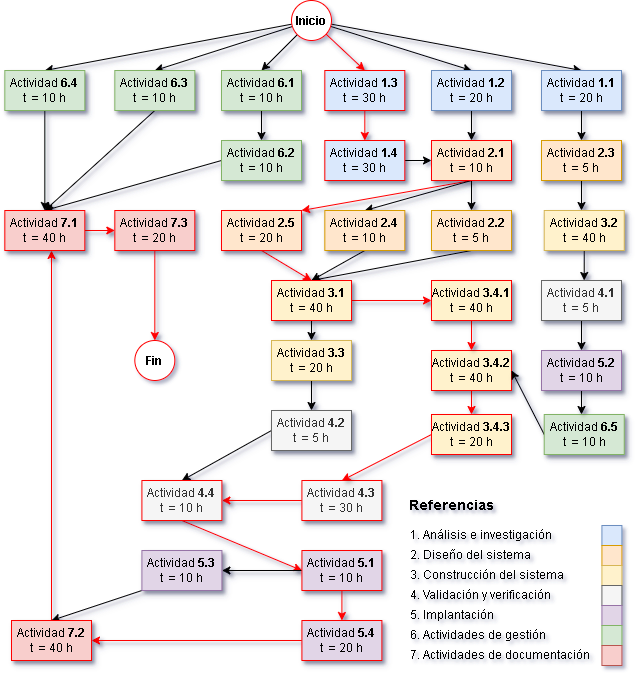
\includegraphics[width=.95\textwidth]{./Figuras/AoN.png}
  \caption{Diagrama de \textit{Activity on Node}.}
  \label{fig:AoN}
\end{figure}

\section{11. Diagrama de Gantt}
\label{sec:gantt}

En la figura \ref{fig:diagGanttAct} se puede observar la lista de actividades, y en la figura \ref{fig:diagGantt} el diagrama Gantt asociado a dicha lista.

\begin{figure}[htpb]
  \centering
  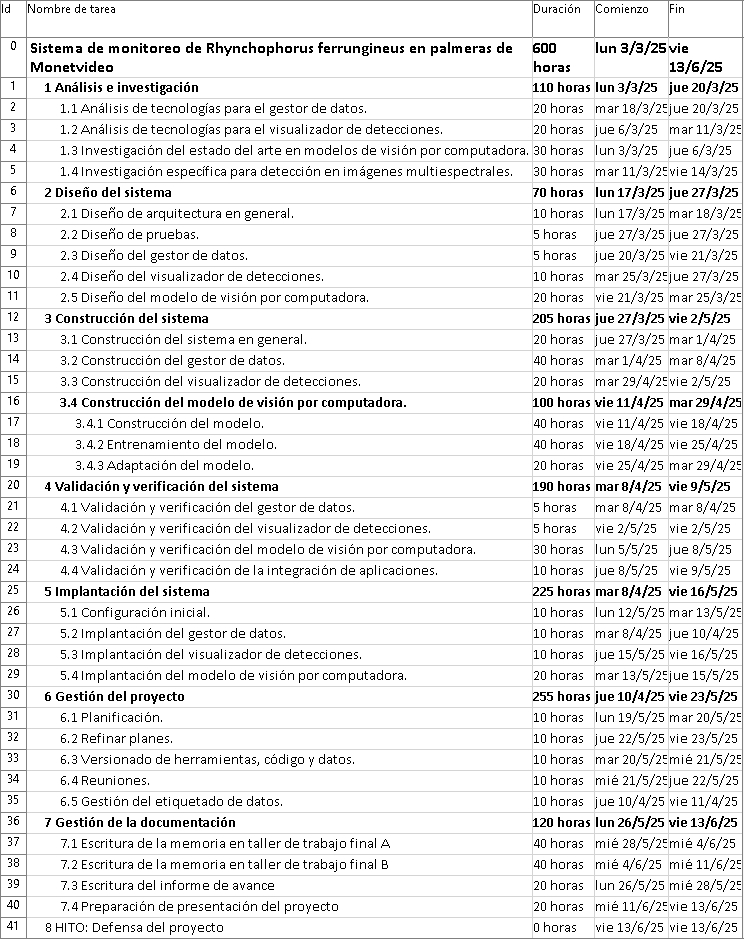
\includegraphics[height=.7\textheight]{./Figuras/lista-actividades.png}
  \caption{Lista de tareas para el Diagrama Gantt.}
  \label{fig:diagGanttAct}
\end{figure}

\begin{landscape}
  \centering
  \vspace*{\fill}
  \begin{figure}[htpb]
    \centering
    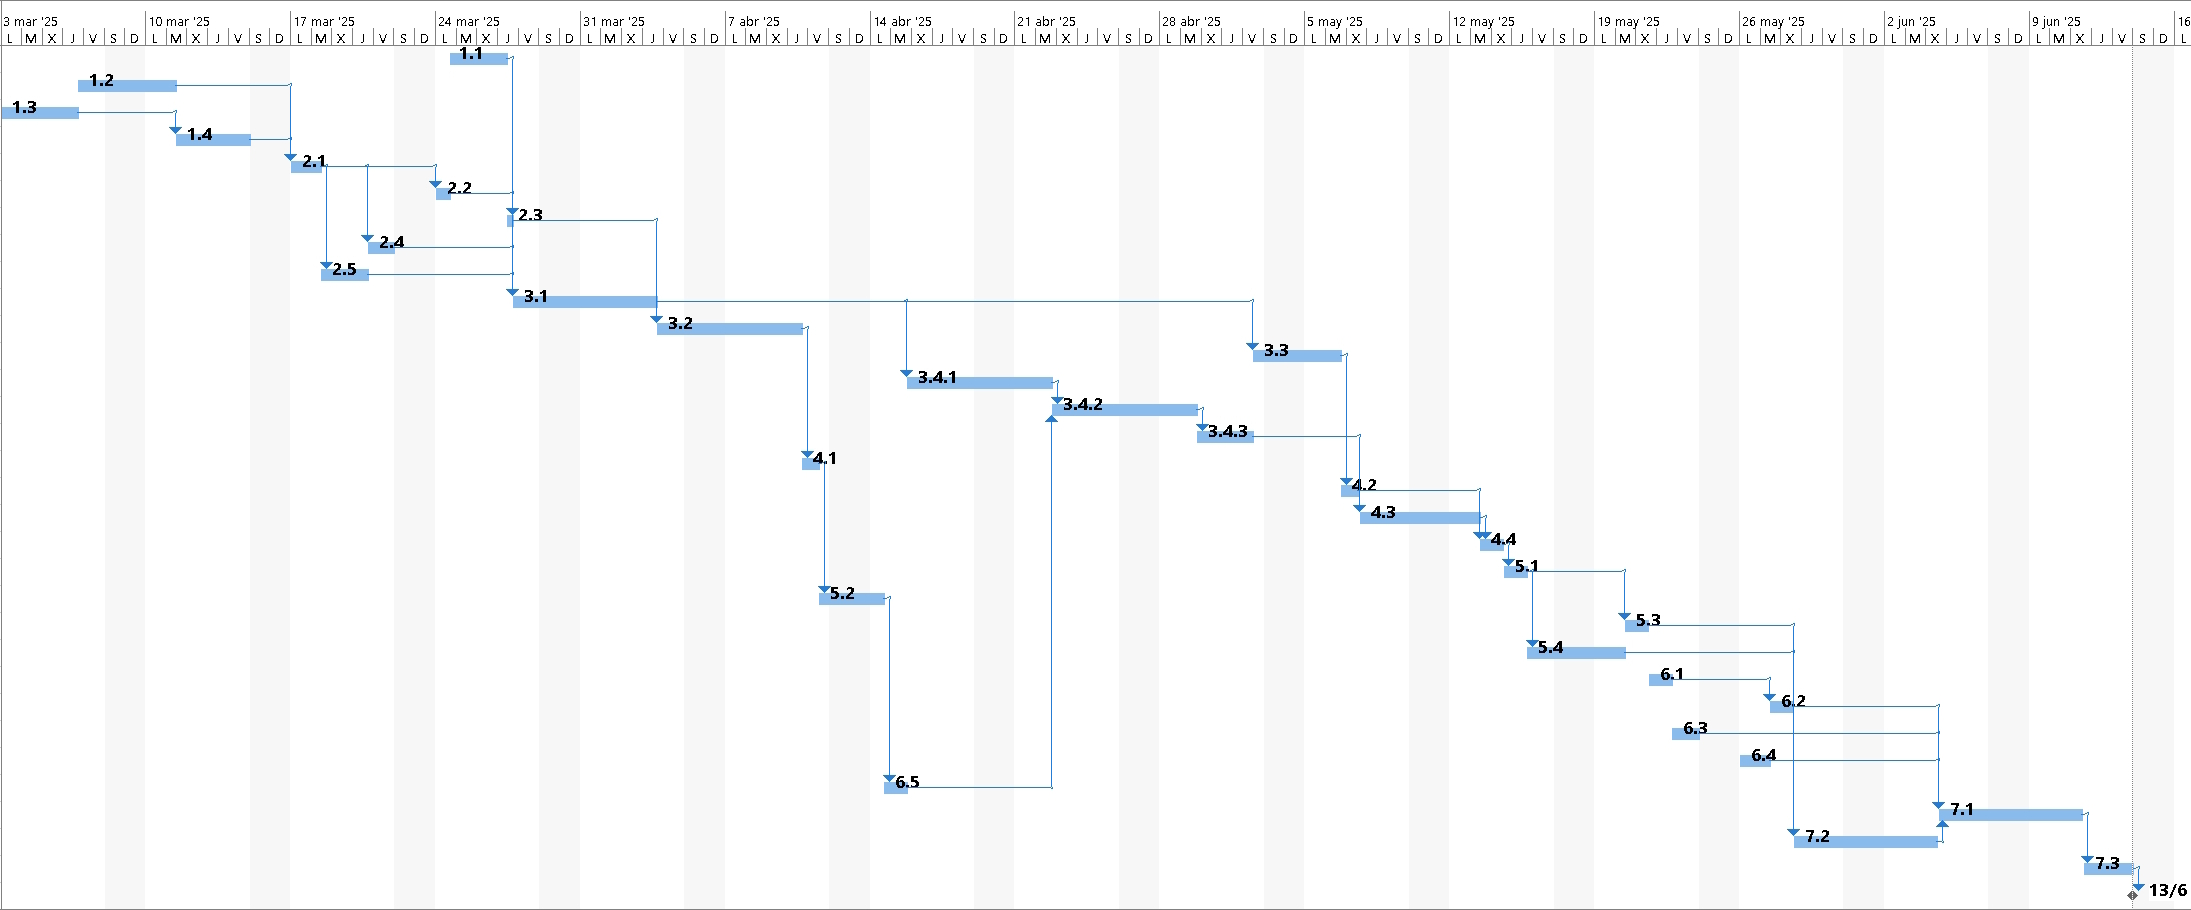
\includegraphics[height=.65\textheight]{./Figuras/gantt.jpg}
    \caption{Diagrama de Gantt.}
    \label{fig:diagGantt}
  \end{figure}
  \vfill
\end{landscape}


\section{12. Presupuesto detallado del proyecto}
\label{sec:presupuesto}

Los principales costos asociados de este proyecto se encuentran en las horas de ingeniería dedicas. Como costos secundarios, las horas de personal cualificado para la realización del etiquetado de los datos. Como punto final, los datos ya se encuentran disponibles, sin embargo, es posible solicitarlos a demanda, por lo que estos costos indirectos también son incluidos.

\begin{table}[htpb]
  \centering
  \begin{tabularx}{\linewidth}{@{}|X|c|r|r|@{}}
    \hline
    \rowcolor[HTML]{C0C0C0}
    \multicolumn{4}{|c|}{\cellcolor[HTML]{C0C0C0}COSTOS DIRECTOS}   \\ \hline

    \rowcolor[HTML]{C0C0C0} Descripción                         &
    \multicolumn{1}{c|}{\cellcolor[HTML]{C0C0C0}Cantidad}       &
    \multicolumn{1}{c|}{\cellcolor[HTML]{C0C0C0}Valor unitario} &
    \multicolumn{1}{c|}{\cellcolor[HTML]{C0C0C0}Valor total}        \\ \hline

    Horas de ingeniería                                         &
    \multicolumn{1}{c|}{600 h}                                  &
    \multicolumn{1}{c|}{USD 30 / h}                             &
    \multicolumn{1}{c|}{USD 18000}                                  \\ \hline

    Horas de cómputo                                            &
    \multicolumn{1}{c|}{100 h}                                  &
    \multicolumn{1}{c|}{USD 0.1}                                &
    \multicolumn{1}{c|}{USD 10}                                     \\ \hline

    Infraestructura y almacenamiento                            &
    \multicolumn{1}{c|}{300 h}                                  &
    \multicolumn{1}{c|}{USD 0.1}                                &
    \multicolumn{1}{c|}{USD 30}                                     \\ \hline

    \multicolumn{3}{|c|}{SUBTOTAL}                              &
    \multicolumn{1}{c|}{USD 18040}                                  \\ \hline
    \rowcolor[HTML]{C0C0C0}
    \multicolumn{4}{|c|}{\cellcolor[HTML]{C0C0C0}COSTOS INDIRECTOS} \\ \hline

    \rowcolor[HTML]{C0C0C0} Descripción                         &
    \multicolumn{1}{c|}{\cellcolor[HTML]{C0C0C0}Cantidad}       &
    \multicolumn{1}{c|}{\cellcolor[HTML]{C0C0C0}Valor unitario} &
    \multicolumn{1}{c|}{\cellcolor[HTML]{C0C0C0}Valor total}        \\ \hline

    Horas de etiquetado                                         &
    \multicolumn{1}{c|}{40 h}                                   &
    \multicolumn{1}{c|}{USD 25}                                 &
    \multicolumn{1}{c|}{USD 1000}                                   \\ \hline

    Vuelos de drones                                            &
    \multicolumn{1}{c|}{5 U}                                    &
    \multicolumn{1}{c|}{USD 500}                                &
    \multicolumn{1}{c|}{USD 2500}                                   \\ \hline

    Imprevistos (40\% costos directos)                          &
    \multicolumn{1}{c|}{1 U}                                    &
    \multicolumn{1}{c|}{USD 7216}                               &
    \multicolumn{1}{c|}{USD 7216}                                   \\ \hline

    \multicolumn{3}{|c|}{SUBTOTAL}                              &
    \multicolumn{1}{c|}{USD 10716}                                  \\ \hline
    \rowcolor[HTML]{C0C0C0}
    \multicolumn{3}{|c|}{TOTAL}                                 &

    USD 28756                                                       \\ \hline
  \end{tabularx}%
\end{table}


\section{13. Gestión de riesgos}
\label{sec:riesgos}

\begin{consigna}{red}
  a) Identificación de los riesgos (al menos cinco) y estimación de sus consecuencias:

  Riesgo 1: detallar el riesgo (riesgo es algo que si ocurre altera los planes previstos de forma negativa)
  \begin{itemize}
    \item Severidad (S): mientras más severo, más alto es el número (usar números del 1 al 10).\\
          Justificar el motivo por el cual se asigna determinado número de severidad (S).
    \item Probabilidad de ocurrencia (O): mientras más probable, más alto es el número (usar del 1 al 10).\\
          Justificar el motivo por el cual se asigna determinado número de (O).
  \end{itemize}

  Riesgo 2:
  \begin{itemize}
    \item Severidad (S): X.\\
          Justificación...
    \item Ocurrencia (O): Y.\\
          Justificación...
  \end{itemize}

  Riesgo 3:
  \begin{itemize}
    \item Severidad (S):  X.\\
          Justificación...
    \item Ocurrencia (O): Y.\\
          Justificación...
  \end{itemize}


  b) Tabla de gestión de riesgos:      (El RPN se calcula como RPN=SxO)

  \begin{table}[htpb]
    \centering
    \begin{tabularx}{\linewidth}{@{}|X|c|c|c|c|c|c|@{}}
      \hline
      \rowcolor[HTML]{C0C0C0}
      Riesgo & S & O & RPN & S* & O* & RPN* \\ \hline
             &   &   &     &    &    &      \\ \hline
             &   &   &     &    &    &      \\ \hline
             &   &   &     &    &    &      \\ \hline
             &   &   &     &    &    &      \\ \hline
             &   &   &     &    &    &      \\ \hline
    \end{tabularx}%
  \end{table}

  Criterio adoptado:

  Se tomarán medidas de mitigación en los riesgos cuyos números de RPN sean mayores a...

  Nota: los valores marcados con (*) en la tabla corresponden luego de haber aplicado la mitigación.

  c) Plan de mitigación de los riesgos que originalmente excedían el RPN máximo establecido:

  Riesgo 1: plan de mitigación (si por el RPN fuera necesario elaborar un plan de mitigación).
  Nueva asignación de S y O, con su respectiva justificación:
  \begin{itemize}
    \item Severidad (S*): mientras más severo, más alto es el número (usar números del 1 al 10).
          Justificar el motivo por el cual se asigna determinado número de severidad (S).
    \item Probabilidad de ocurrencia (O*): mientras más probable, más alto es el número (usar del 1 al 10).
          Justificar el motivo por el cual se asigna determinado número de (O).
  \end{itemize}

  Riesgo 2: plan de mitigación (si por el RPN fuera necesario elaborar un plan de mitigación).

  Riesgo 3: plan de mitigación (si por el RPN fuera necesario elaborar un plan de mitigación).

\end{consigna}


\section{14. Gestión de la calidad}
\label{sec:calidad}

\begin{consigna}{red}
  Elija al menos diez Requisitos que a su criterio sean los más importantes/críticos/que aportan más valor y para cada uno de ellos indique las acciones de verificación y validación que permitan asegurar su cumplimiento.

  \begin{itemize}
    \item Req \#1: copiar acá el requerimiento con su correspondiente número.

          \begin{itemize}
            \item Verificación para confirmar si se cumplió con lo requerido antes de mostrar el sistema al cliente. Detallar.
            \item Validación con el cliente para confirmar que está de acuerdo en que se cumplió con lo requerido. Detallar.
          \end{itemize}

  \end{itemize}

  Tener en cuenta que en este contexto se pueden mencionar simulaciones, cálculos, revisión de hojas de datos, consulta con expertos, mediciones, etc.

  Las acciones de verificación suelen considerar al entregable como ``caja blanca'', es decir se conoce en profundidad su funcionamiento interno.

  En cambio, las acciones de validación suelen considerar al entregable como ``caja negra'', es decir, que no se conocen los detalles de su funcionamiento interno.

\end{consigna}

\section{15. Procesos de cierre}
\label{sec:cierre}

\begin{consigna}{red}
  Establecer las pautas de trabajo para realizar una reunión final de evaluación del proyecto, tal que contemple las siguientes actividades:

  \begin{itemize}
    \item Pautas de trabajo que se seguirán para analizar si se respetó el Plan de Proyecto original:\\
          - Indicar quién se ocupará de hacer esto y cuál será el procedimiento a aplicar.
    \item Identificación de las técnicas y procedimientos útiles e inútiles que se emplearon, los problemas que surgieron y cómo se solucionaron:\\
          - Indicar quién se ocupará de hacer esto y cuál será el procedimiento para dejar registro.
    \item Indicar quién organizará el acto de agradecimiento a todos los interesados, y en especial al equipo de trabajo y colaboradores:\\
          - Indicar esto y quién financiará los gastos correspondientes.
  \end{itemize}

\end{consigna}

\bibliographystyle{unsrt} % Elige el estilo de cita (plain, alpha, apa, etc.)
\bibliography{charter} % Nombre del archivo .bib sin extensión

\end{document}